\documentclass[conference]{IEEEtran}
\usepackage{cite}
\usepackage{amsmath,amssymb,amsfonts}
\usepackage{algorithmic}
\usepackage{graphicx}
\usepackage{textcomp}
\usepackage{xcolor}
\def\BibTeX{{\rm B\kern-.05em{\sc i\kern-.025em b}\kern-.08em
    T\kern-.1667em\lower.7ex\hbox{E}\kern-.125emX}}
\begin{document}

\title{A Latent World Model for Action-Conditioned Prediction in Interactive 2D Physics Environments}

\author{
\IEEEauthorblockN{Danilo César Tertuliano Melo}
\IEEEauthorblockA{
\textit{Universidade de Brasília} \\
Brasília, Brazil \\
daniloctmelo@gmail.com
}
\and
\IEEEauthorblockN{Felipe Lopes Gibin Duarte}
\IEEEauthorblockA{
\textit{Universidade de Brasília} \\
Brasília, Brazil \\
gibinf.duarte@gmail.com
}
\and
\IEEEauthorblockN{Matheus de Melo Fellet}
\IEEEauthorblockA{
\textit{Universidade de Brasília} \\
Brasília, Brazil \\
matheusmfellet@gmail.com
}
\and
\IEEEauthorblockN{Yuri Santana Lopes}
\IEEEauthorblockA{
\textit{Universidade de Brasília} \\
Brasília, Brazil \\
yuri03ysl@gmail.com
}
}

\maketitle

\begin{abstract}
World models offer a powerful paradigm for learning the internal representations and temporal dynamics of complex environments directly from high-dimensional sensory data. This paper presents a modular latent world model designed to predict the visual evolution of a two-dimensional physical simulation conditioned on external user interventions. To overcome the computational inefficiency and instability associated with direct pixel-space prediction, the proposed architecture decomposes the forecasting problem into visual compression, action embedding, multimodal fusion, and latent dynamics prediction. A Variational Autoencoder (VAE) is employed to compress individual $64 \times 64$ grayscale frames into a structured spatial latent space. Concurrently, an Action Encoder maps user interactions, specifically the instantaneous spawning of objects at given coordinates, into continuous latent vectors. These representations are combined via spatial broadcast fusion and fed into a transition predictor that estimates the subsequent latent state based on a stacked temporal history of past observations. Trained on a custom synthetic dataset generated via a 2D physics engine, the proposed framework is evaluated on held-out episodes against trivial baselines and a reconstruction oracle. The subsequente ball position is more accurately predicted than persistence and constant-velocity extrapolation across all test epides, responding specifically and locally to user interventions, and captures the direction of gravity-driven motion more reliably than magnitude. These results indicate that the model abstracts basic aspects of gravity-driven dynamics and localized interventions, providing a foundational approach for action-conditioned generative prediction in interactive physical enviroments.
\end{abstract}

\begin{IEEEkeywords}
World Models; Model-Based Reinforcement Learning; Action-Conditioned Prediction; Latent Dynamics; Synthetic Physics Environments.
\end{IEEEkeywords}

\section{Introduction}
\label{sec:introduction}

World models are generative models that aim to learn an internal representation of an environment and its temporal dynamics from observed experience. Instead of operating directly on high-dimensional sensory data, such as images or raw pixel observations, these models typically encode observations into a compact latent space in which the relevant spatial and temporal structure of the environment can be represented more efficiently. In this sense, a world model serves as an abstract simulator of the environment, allowing an agent or predictive system to estimate future states based on previous observations and actions \cite{ha2018world, hafner2019learning}.

In model-based learning, world models are particularly useful because they enable prediction, planning, and policy learning through imagined trajectories rather than relying exclusively on direct interaction with the real environment. Works such as PlaNet \cite{hafner2019learning} and Dreamer \cite{hafner2020dream} demonstrate that learning dynamics in latent space can support long-horizon reasoning from visual inputs, allowing agents to simulate possible futures and evaluate the consequences of actions before executing them. More recently, this paradigm has scaled towards overarching platforms for 'Physical AI', such as the Cosmos World Foundation Model \cite{agarwal2025cosmos}, which emphasizes the necessity of foundational models that inherently grasp complex physical laws and spatial dynamics. Therefore, in the context of this work, a world model can be understood as a latent generative model that learns the physical evolution of a simulated environment and predicts its next visual state conditioned on both the history of observations and external interventions.

The main contribution of this work is the development of a latent world model for predicting the visual evolution of a two-dimensional physical simulation conditioned on external user interventions. Unlike approaches that model future frames directly in pixel space, the proposed architecture separates the problem into visual compression, latent dynamics prediction, and visual reconstruction, enabling the system to learn a compact representation of the environment before modeling its temporal evolution. By combining a visual encoder, an action embedding module, a latent transition model, and a decoder, the proposed method investigates how physical interactions, such as gravity and collisions between circular bodies, can be learned in a structured latent space. This formulation provides a foundation for studying action-conditioned generative prediction in controlled physical environments and contributes to the broader development of world models capable of simulating future states from visual observations and interventions.

\section{Problem Formulation}
\label{sec:problem_formulation}

The objective of this work is to develop a generative model capable of predicting the evolution of a two-dimensional physical environment conditioned on external actions. More specifically, the goal is to estimate the next visual state of a simulation containing multiple balls subject to gravity and collisions, considering both the natural dynamics of the system and an intervention performed by the user.

The environment is represented as a temporal sequence of frames. Each frame corresponds to the complete visual state of the simulation at a given time step. Let \(x_t \in \mathbb{R}^{H \times W \times C}\) denote the observed frame at time \(t\), where \(H\) and \(W\) represent the height and width of the image, respectively, and \(C\) represents the number of channels. The input to the model consists of a temporal window containing the last \(k\) observed frames:

\begin{equation}
    X_t = \{x_{t-k+1}, x_{t-k+2}, \ldots, x_{t-1}, x_t\}.
\end{equation}

In addition to the visual sequence, the model receives an action \(a_t\), which is responsible for modifying the environment. In this work, actions correspond to the insertion of a new ball at specific coordinates in the scene. Thus, an action can be represented as a 4-dimensional vector:

\begin{equation}
    a_t = (v_{{\text{type}},t}, v_{{\text{obj}},t}, p^x_t, p^y_t),
\end{equation}

where $v_{{\text{type}},t} \in \{0.0, 1.0\}$ indicates the presence of an action (\texttt{mouse\_down} vs. \texttt{none}), $v_{{\text{obj}},t} \in \{0.0, 1.0\}$ encodes the type of object being introduced (\texttt{ball} vs. \texttt{none}), and $p^x_t, p^y_t \in [0,1]$ represent the normalized spatial coordinates of the interaction relative to the dimensions of the screen ($800 \times 600$). 

In the current experimental configuration, all physical and material properties of the system are kept strictly uniform. Specifically, the radius, mass, surface friction, and elasticity of the object remain constant across all instances and are thus omitted from the action embedding.

Due to the high dimensionality of the pixel space, direct modeling of the conditional distribution $P(x_{t+1} \mid x_{1:t}, a_t)$ is computationally expensive and prone to instability. Therefore, we adopt the fundamental premise of world models: the dynamics of the world can be represented in a more compact latent space.

The problem is therefore decomposed into three interdependent subproblems:

\subsection{Spatial Compression: Visual Perception}

The first step consists of reducing the dimensionality of the visual data. Instead of computing the dynamics directly over thousands of pixels, we seek to map each high-dimensional frame $x_t$ to a more compact and information-dense latent representation, denoted by $z_t$. To ensure a smooth and continuous latent space that facilitates the learning of temporal dynamics, this spatial compression is implemented using a Variational Autoencoder (VAE) \cite{kingma2013autoencoding}.

During its independent training phase, the VAE employs a probabilistic approach. The encoder function $E$ outputs the parameters of a multivariate Gaussian distribution, specifically the mean vector $\mu_t$ and the log-variance vector $\sigma_t^2$:

\begin{equation}
    (\mu_t, \log \sigma_t^2) = E(x_t).
\end{equation}

The network is optimized by sampling a latent vector $z_t$ using the reparameterization trick ($z_t = \mu_t + \sigma_t \odot \epsilon$, where $\epsilon \sim \mathcal{N}(0, I)$ and $\sigma_t = \exp(0.5 \log(\sigma_t^2))$). This formulation preserves end-to-end differentiability during training and encourages the latent space to remain smooth and continuous.

However, once the VAE is trained and deployed as a feature extractor for the World Foundation Model, we adopt a deterministic approach. To avoid injecting stochastic noise into the physics modeling, the latent representation of the frame is taken directly as the expected value of the distribution:

\begin{equation}
    z_t = \mu_t.
\end{equation} 

The purpose of this compression is to extract the fundamental characteristics of the scene, such as the spatial positions of the balls and the geometry of the environment, while discarding visual redundancies and noise. By stacking the latent representations of the last $k$ frames, we obtain the latent state history of the system, denoted by $Z_t$:

\begin{equation}
    Z_t = \{z_{t-k+1}, z_{t-k+2}, \ldots, z_{t-1}, z_t\}.
\end{equation}

\subsection{Latent Dynamics Prediction: World Modeling}

The core of the problem lies in learning the rules of physics, such as gravity, inertia, and collisions, in the latent space. In order for the model to understand user interventions, the action \(a_t\) is also mapped to a continuous numerical feature space through an embedding function, resulting in a representation \(e_t\):

\begin{equation}
    e_t = A(a_t),
\end{equation}

where \(A\) denotes the action embedding function.

The world model acts as a fully latent neural simulator. It defines a transition function \(W\), which receives the compressed visual history and the applied action, and attempts to predict the latent state at the next time step:

\begin{equation}
    \hat{z}_{t+1} = W(Z_t, e_t).
\end{equation}

It is in this stage that the system reasons about time and causality, determining the direction and velocity of the objects based on the provided temporal history.

\subsection{Visual Reconstruction of the Next Frame}

Finally, in order for the prediction to be interpretable and visually comparable to the real environment, the predicted latent state \(\hat{z}_{t+1}\) must be translated back into the original pixel space. This is performed by a decoder function \(D\), which maps the latent representation into a visible image:

\begin{equation}
    \hat{x}_{t+1} = D(\hat{z}_{t+1}).
\end{equation}

Thus, the problem formulation is defined in two main optimization stages. In the first stage, the focus is on optimizing the encoder \(E\) and decoder \(D\), so that the system can accurately represent the environment in the latent space and reconstruct it in the pixel space. In the second stage, once the spatial latent representation is well established, the focus shifts to the transition function \(W\), whose objective is to minimize the divergence between the predicted latent state \(\hat{z}_{t+1}\) and the true encoding of the next observed frame \(E(x_{t+1})\).

\section{Dataset}
\label{sec:dataset}

In order for the world model to learn how to represent the physics of the environment and respond to external commands, it was necessary to construct a more controlled dataset. The choice of synthetic data, rather than real-world videos, is justified by the need to isolate fundamental variables such as gravity, collision, and inertia from complex visual noise, including variable lighting, complex textures, and arbitrary occlusions, which could obscure the learning of purely mechanical dynamics.

\subsection{Simulation Environment}

The environment was built using the Pymunk 2D physics engine \cite{pymunk}, a Python interface for the Chipmunk2D library \cite{chipmunk2d}, which is capable of simulating fundamental mechanical properties in a deterministic manner. The basic scenario consists of a space with a floor and no walls, where physical interactions occur, as illustrated in Fig. \ref{fig:simulation_environment}.

\begin{figure}[!h]
    \centering
    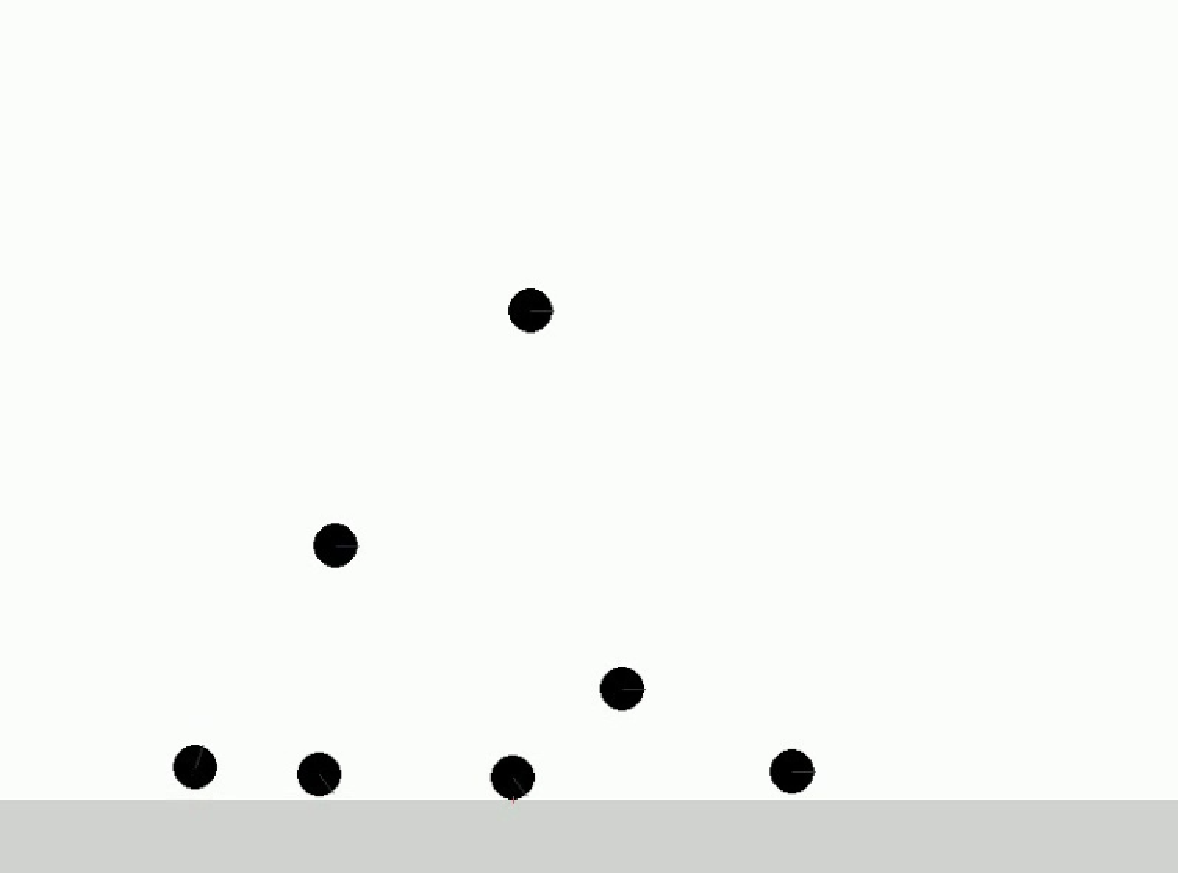
\includegraphics[width=\columnwidth]{figures/simulationEnvironment.pdf}
    \caption{Example frame from the simulated physical environment used for data generation. The scene contains multiple interacting objects whose dynamics are governed by the physics engine.}
    \label{fig:simulation_environment}
\end{figure}

The main dynamics of the environment involve circular objects that fall under the effect of gravity, collide with the floor and with each other, bounce with partial conservation of elastic energy, and eventually reach a resting state due to friction. The distinguishing feature of this environment is its interactivity: at any moment, an external intervention may occur in the form of a user ``click'' action, which instantly creates a new object at a specific coordinate on the screen, thereby altering the natural course of the simulation.

\subsection{Data Generation}

Data collection was automated through a set of procedural simulations, referred to as \textit{episodes}. Each episode consists of a short temporal sequence in which multiple actions are triggered at random times and positions, ensuring broad coverage of the state space. The generation process produces two synchronized data streams:

\begin{itemize}
    \item \textbf{Video:} The visual record of the simulation, rendered at a fixed rate of 60 frames per second (FPS). To reduce computational cost and focus on shape rather than color, the original frames, generated at higher resolutions such as \(800 \times 600\), are resized to \(64 \times 64\) pixels, converted to grayscale, and normalized to the interval \([0, 1]\).

    \item \textbf{Event Log:} A file in JavaScript Object Notation (JSON) format that records the exact time at which each action occurred and its corresponding properties. This log is used as input to automatically generate the video sequence.
\end{itemize}

An important detail in preparing these data for the temporal model is the construction of the frame history. Since the model requires a window of \(k\) frames, the initial time steps of the video, which do not have sufficient previous context, are padded by replicating the first available frame.

\subsection{Action Representation}

In a continuous simulation scenario, most frames occur without any external intervention. Therefore, the action representation needed to consistently handle both the moment of the click and the natural inertia of the environment.

Based on the event log, actions were extracted and aligned with the video frames using the timestamps and the fixed frame rate.

For frames in which the user does not perform any interaction, the system generates a \textit{Null Action}, represented by a zero vector corresponding to the absence of external intervention. This modeling choice is important because it teaches the model that, in the absence of an external action, it should only propagate the natural physics inferred from the previous frames.

\section{Proposed Model}
\label{sec:proposed_model}

The general architecture of this world model is organized as a modular pipeline designed to learn the dynamics of 2D physical scenes from simulations and structured actions, as illustrated in Fig.~\ref{fig:world_model_architecture}. Initially, scripts based on Pymunk and Pygame generate the physical scenarios, producing simulation videos and JSON files containing the actions executed over time. These videos go through a preprocessing stage, where they are converted into $64 \times 64$ grayscale frames. Then, a VAE is used to compress each frame into a compact visual latent representation, allowing the model to operate in a lower-dimensional space instead of working directly with image pixels.

\begin{figure}[!h]
    \centering
    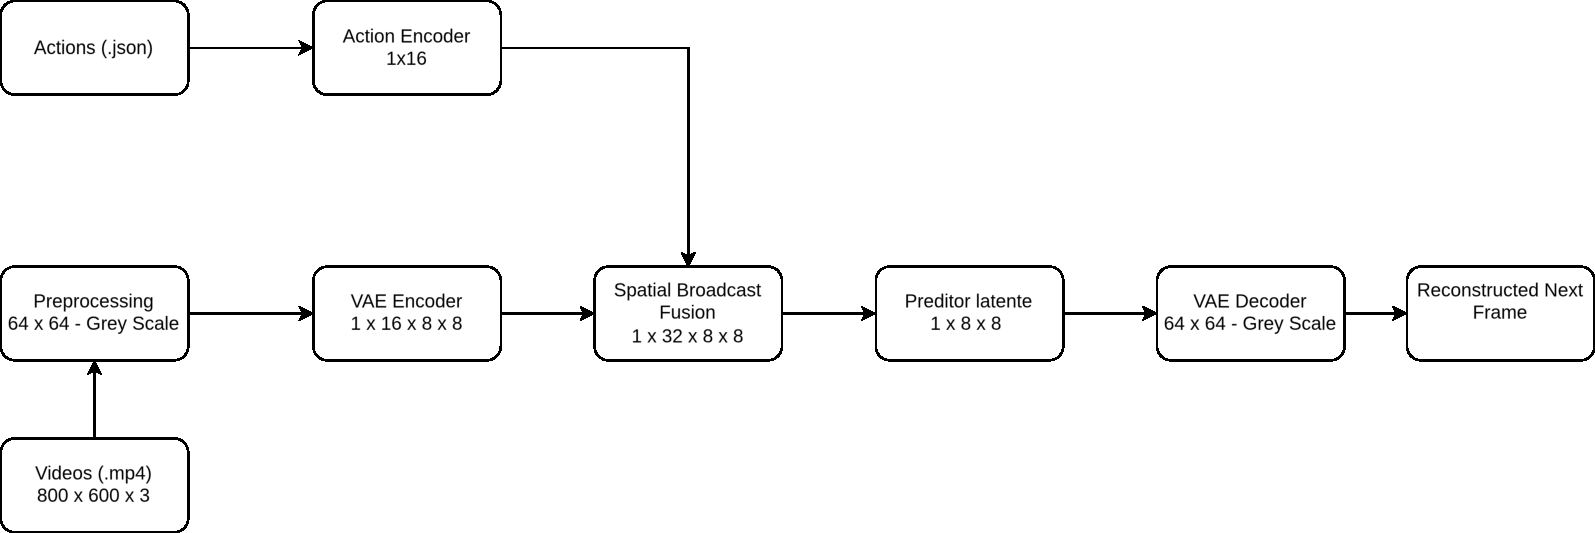
\includegraphics[width=\columnwidth]{figures/worldModel.pdf}
    \caption{Architecture of the proposed world model.}
    \label{fig:world_model_architecture}
\end{figure}

In parallel, each agent action is represented in a structured format using attributes such as action type, target object, and spatial coordinates. The action is encoded by an Action Encoder into a continuous latent vector, which is later combined with the visual representation through spatial broadcast fusion, inspired by the Spatial Broadcast Decoder architecture proposed in \cite{watters2019spatial}. In this process, the action embedding is replicated across the spatial dimensions of the visual feature map and concatenated with the visual features at every location. This enables the predictor to condition its representation of the scene dynamics on the agent's action while preserving the spatial structure of the scene. The resulting fused representation contains information about both the current state of the environment and the intervention performed by the agent.

From this representation, a predictor model learns to estimate the next visual state in latent space, which is then decoded by the VAE Decoder to reconstruct the next simulation frame. In this way, the architecture separates the problem into specialized components: visual representation, action representation, multimodal fusion, and prediction of the world's evolution.


\section{Experimental Setup}
\label{sec:experimental_setup}

Our experiments aim to verify two central hypotheses:
\begin{itemize}
    \item (\textit{H1})~the model learns underlying physical dynamics (e.g., gravity, collisions) rather than merely memorizing trajectories;
    \item (\textit{H2})~its predictions are genuinely conditioned by user interventions, independently of inertial cues already present in the visual context.
\end{itemize}

\subsection{Held-Out Evaluation Set}

In order to test \textit{H1} against memorization, 24 new episodes were generated after training, using the same engine, action distribution and rendering pipeline of Section~\ref{sec:dataset}, so that any performance difference reflects the unseen trajectories rather than a rendering shift. This yielded $10{,}127$ evaluated transitions, $273$ conditioned by a click. Following (1) and (5), the temporal window holds the $k$ most recent contiguous frames. Sweeping $k \in \{1,2,4,6,8,10,12\}$, the latent skill score (0 matches persistence, 1 is perfect) saturates beyond $k=4$ --- $+0.074$ at $k=6$, $+0.072$ at $k=8$, $+0.070$ at $k=12$ --- so we adopt $k=6$, the choice being uncritical above saturation; $k=1$ collapses it to $-0.803$, an error $80\%$ larger than persistence, confirming that the stacked history is what makes velocity estimable. Each action is assigned to the last frame that does \emph{not} yet contain the spawned ball, i.e.\ $\lceil t \cdot f_s \rceil - 1$ for an event at time $t$ with frame rate $f_s$. This makes \textit{H2} testable: the object is absent from the visual history and its coordinates exist only in the action embedding, so a response correctly \emph{localized} at the clicked position cannot be attributed to visual context.

\subsection{Baselines and Model Variants}

To isolate the contributions of specific components, we evaluate the proposed architecture against several baselines:

\textbf{Trivial baselines:} 

\begin{itemize}
    \item \textbf{Persistence ($x_{t+1} = x_t$):} Repeats the last frame. This exposes the limitations of pixel-level metrics, which can score artificially high because they are dominated by the static background rather than object dynamics.
    \item \textbf{Constant Velocity ($x_{t+1} = \text{clip}(2x_t - x_{t-1}, 0, 1)$):} Assumes uniform linear motion, inherently failing to model acceleration, elastic collisions, or sudden object insertions. Coordinates are normalized to $[0,1]$, and the clip is applied per coordinate.
    \item \textbf{Reconstruction oracle.} The \textit{VAE ceiling} decodes the true next latent, $\hat{x}_{t+1} = D(E(x_{t+1}))$: the error floor set by the autoencoder's reconstruction alone, independent of any prediction. Since this oracle is itself far outperformed by pixel-space persistence, a comparison in pixel space cannot separate prediction from reconstruction; the decoded domain is therefore the primary reference for \textit{H1}, with the pixel-space figures quantifying the cost of the autoencoder.
    \item \textbf{Abalation:}\textit{No-Action} the architecture remains unchanged (Acction Encoder, Spatial-Broadcast Fuser and transition model are all active), but the action input is supressesed by reducing it forcibly to $0$ at every step. Since the network is identical and only the action signal is removed, the gap between the full model and this variant isolates the contribution of the action channel, providing the reference against which action sensitivity is measured for \textit{H2}. 
\end{itemize}

\subsection{Evaluation Metrics}

\subsection{Training and Inference Protocol}

\subsubsection{Model Ablations}

These variants evaluate the structural choices of our architecture:

\begin{itemize}
    \item \textbf{No-Action:} The complete architecture is retained - Action Encoder, Spatial-Broadcast Fuser, and Latent Decoder are all active - but the action input is forced to $\mathbf{0}$ at every time step.
    Because no architectural component is removed, any difference in performance relative to the full model is attributable exclusively to the action signal, providing a direct test of \textit{H2}.
    By construction, the action-sensitivity metric evaluated exactly zero for this variant.
\end{itemize}



\subsection{Evaluation Metrics and Training Protocol}
The evaluation combines standard image fidelity metrics with domain-specific physical metrics, as pixel-level functions (e.g., Mean Squared Error) often fail to capture structural consistency and mass conservation.

Training strictly follows the two-stage decomposition defined in Section~\ref{sec:problem_formulation}. This separates the optimization processes, ensuring the spatial visual representation (VAE) fully converges before the system attempts to learn the complex temporal dynamics (World Model).


\section{Results}
\label{sec:results}

\begin{figure}[!h]
    \centering
    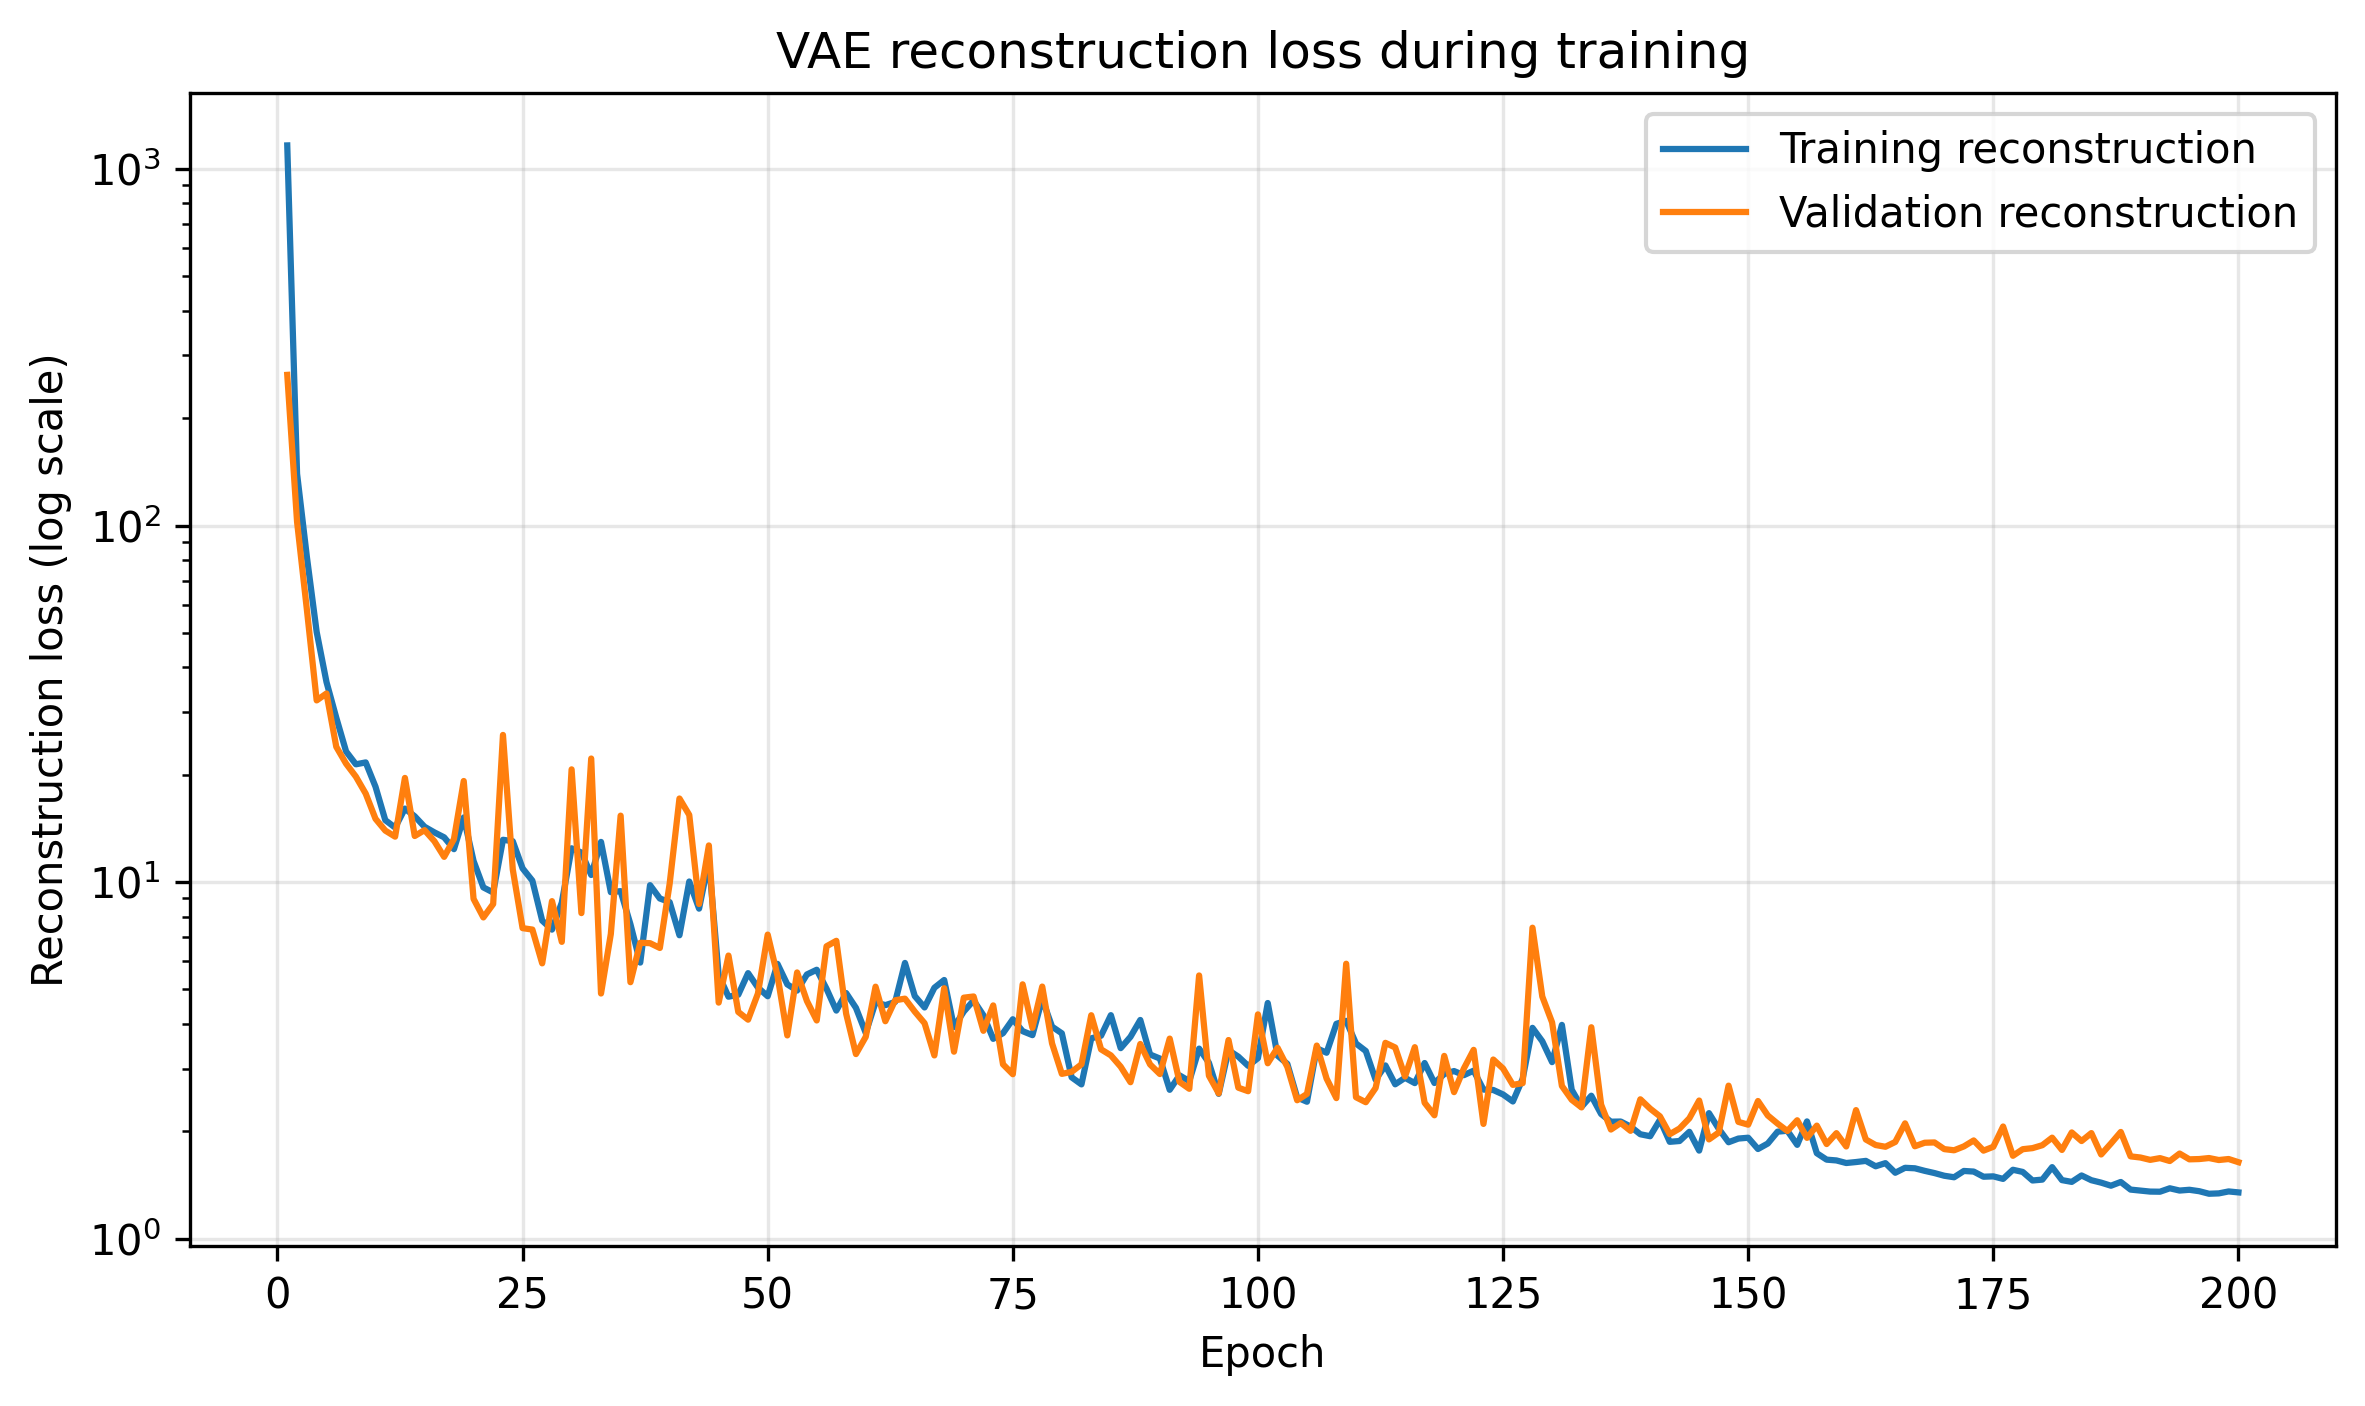
\includegraphics[width=\columnwidth]{figures/vae_reconstruction_loss.png}
    \caption{VAE reconstruction loss during training.}
    \label{fig:vae_reconstruction_loss}
\end{figure}

\begin{figure}[!h]
    \centering
    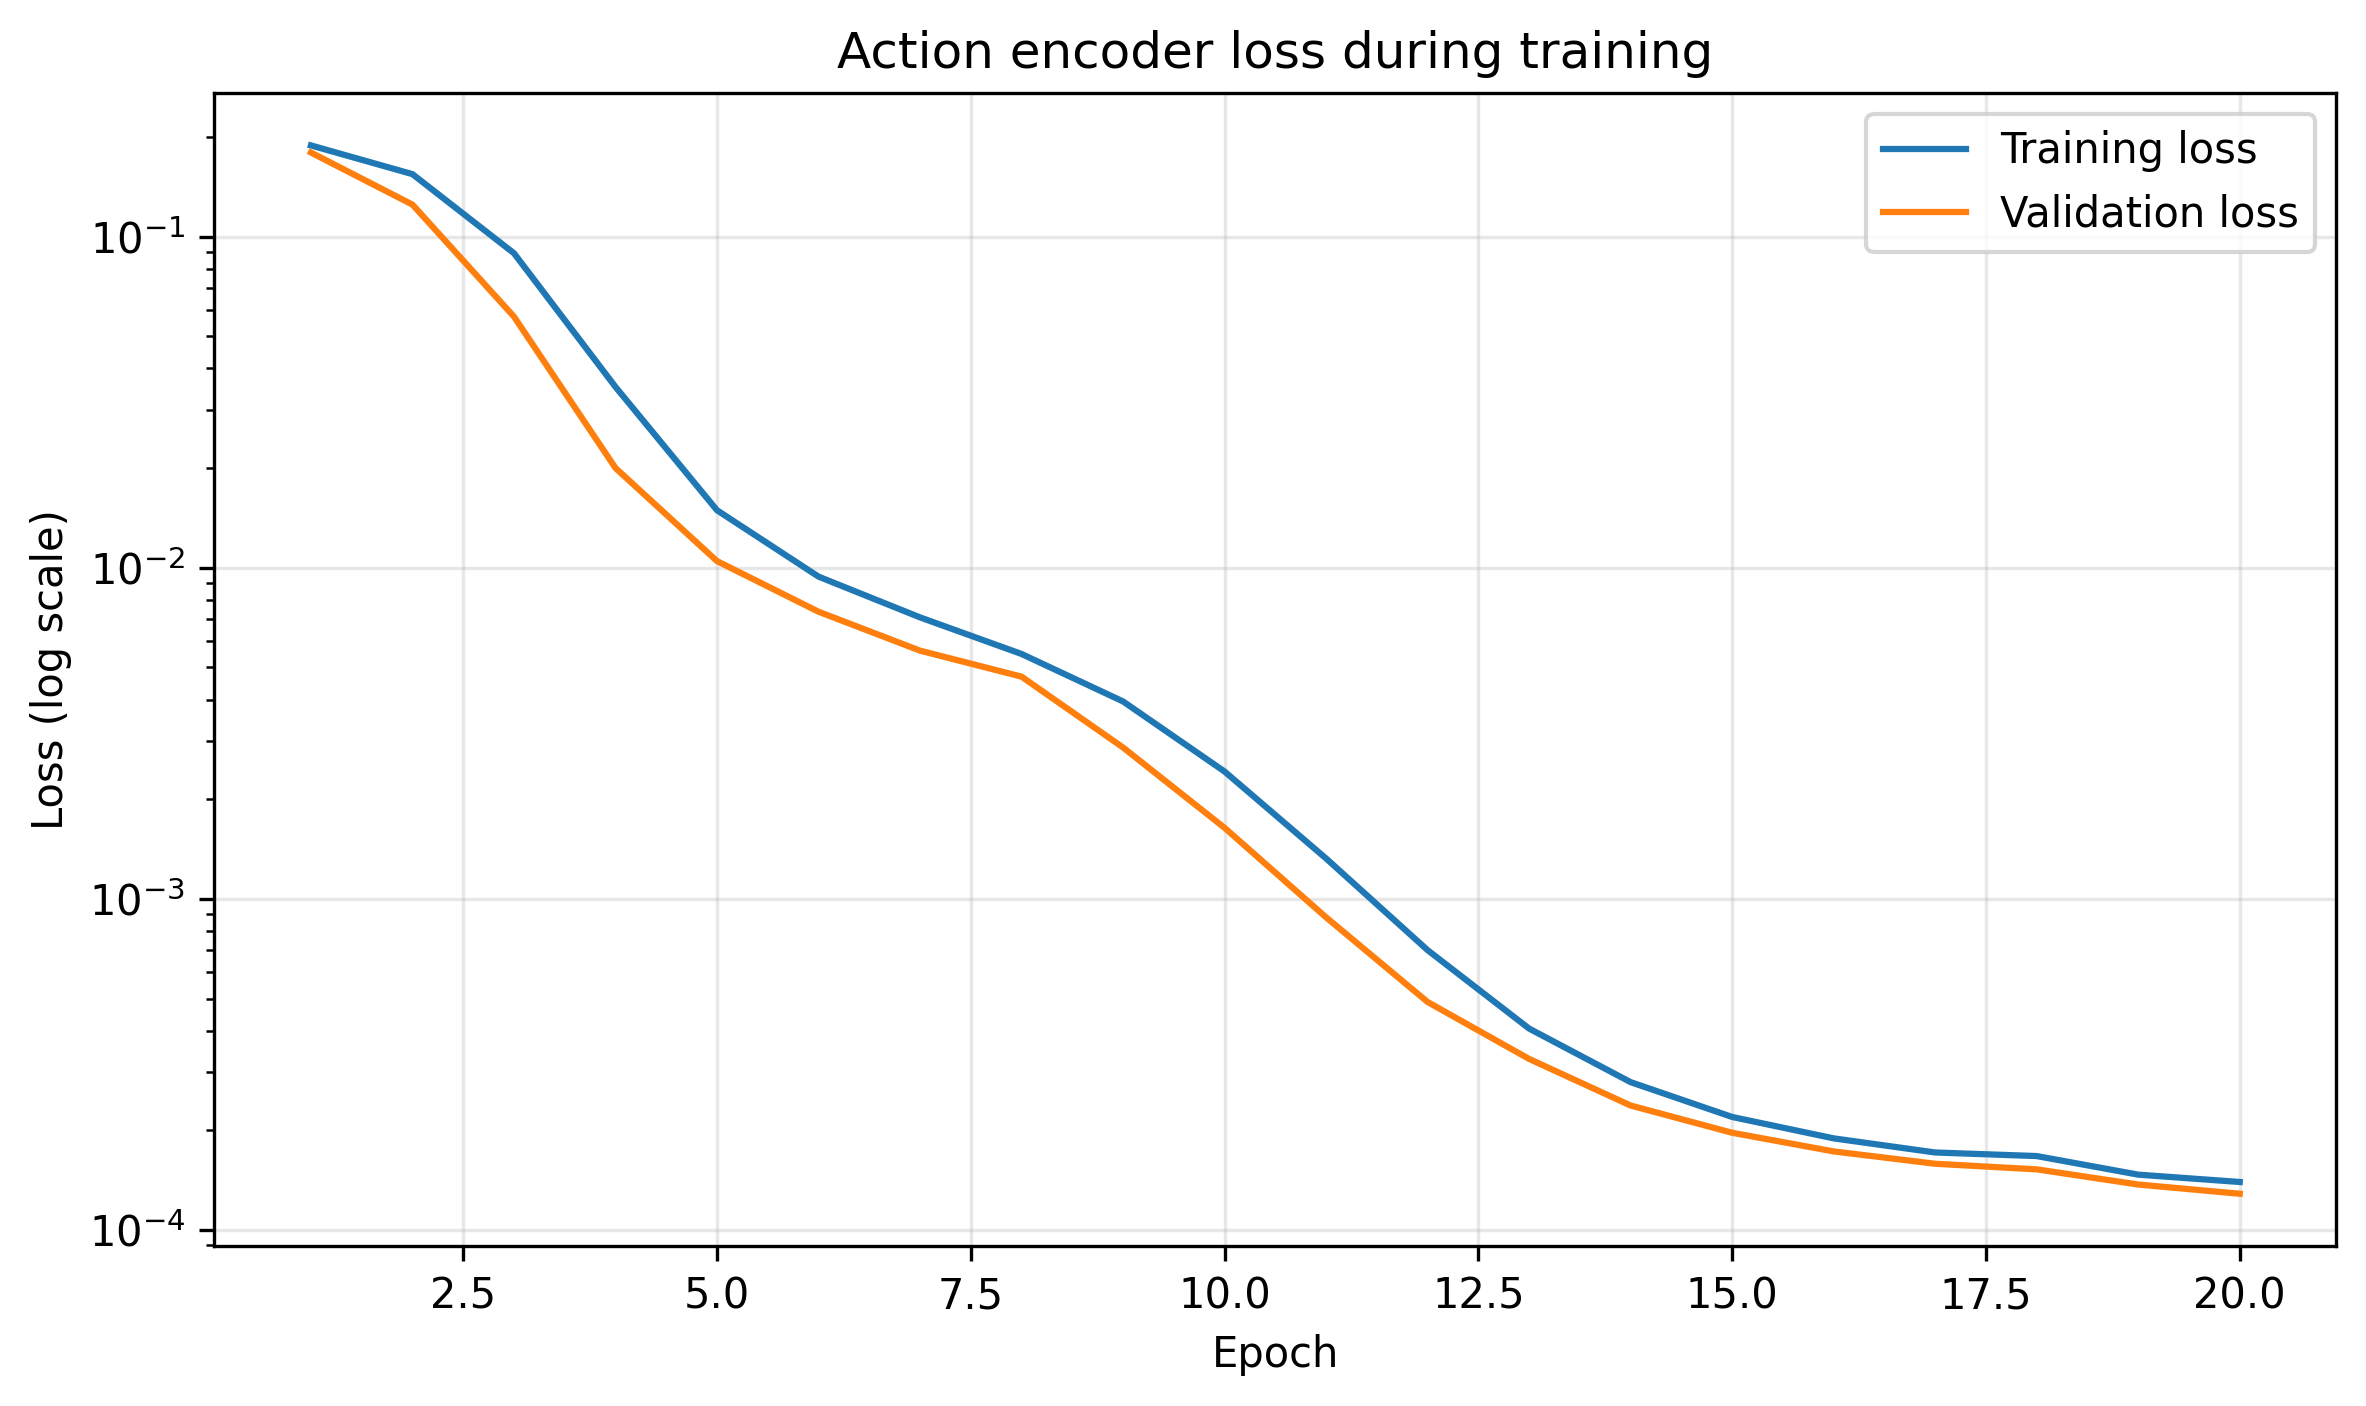
\includegraphics[width=\columnwidth]{figures/action_encoder_loss.png}
    \caption{Action encoder loss during training.}
    \label{fig:action_encoder_loss}
\end{figure}

The internal components of the \textit{world foundation model} were evaluated independently based on the training history of each module. The visual representation module was trained as a variational autoencoder (VAE), while the action encoder was trained to learn a compact representation of the interaction commands. Since these modules optimize different loss functions and operate on different representations, the absolute loss values should not be directly compared. Therefore, the analysis focuses on convergence behavior, validation loss reduction, and the gap between the training and validation curves.

The VAE showed a substantial reduction in loss throughout training. The total training loss decreased from 1170.73 to 1.37 over 200 epochs, while the validation loss decreased from 293.52 to 1.73. The best validation result was obtained in the final epoch, corresponding to a relative validation loss reduction of 99.41\%. The reconstruction component followed the same trend, with the validation reconstruction loss decreasing from 264.52 to 1.64. This behavior indicates that the encoder--decoder structure progressively learned a compact latent representation capable of reconstructing the visual state of the simulated environment. The KL divergence increased during the initial phase and later stabilized in a high-value regime, which is expected after the $\beta$ warm-up phase and suggests that the latent space was effectively regularized without collapsing.

The action encoder presented a highly stable convergence profile. The training loss decreased from 0.1886 to 0.00014, and the validation loss decreased from 0.1795 to 0.00013 over 20 epochs. The best validation value was also achieved in the final epoch, resulting in a relative reduction of 99.93\%. The close alignment between the training and validation curves indicates that the action representation learned by the encoder generalized well to the validation set, with no evidence of overfitting in the observed training history.

Overall, the results support the viability of the modular representation learning strategy adopted in this work. The VAE was able to compress visual observations into a structured latent representation, while the action encoder learned a stable representation for interaction commands. Together, these results indicate that the trained components provide a suitable foundation for subsequent stages of the architecture, in which visual and action representations can be integrated to support future state prediction in the simulated environment.



\bibliographystyle{IEEEtran}
\bibliography{biblio}
\vspace{12pt}

\end{document}